\documentclass[12pt]{article}
\usepackage[letterpaper, margin=1in]{geometry}
\usepackage{setspace}
\usepackage[dvipsnames]{xcolor}
\usepackage{ragged2e}
\usepackage{amsmath}
\usepackage{cancel}
\usepackage{multicol}
\usepackage{multirow}
\usepackage{fancyhdr}
\pagestyle{fancy}
\usepackage{lastpage} 
\usepackage{xcolor,colortbl}
\usepackage{amssymb}
\usepackage{graphicx}

\lhead{April 1, 2021}
\chead{}
\rhead{jnrozano@up.edu.ph}

\lfoot{Jhon Christian N. Rozano}
\cfoot{}
\rfoot{Page \thepage\ of \pageref{LastPage}}

\renewcommand{\headrulewidth}{1pt}

\renewcommand{\footrulewidth}{1pt}

\newcommand*\Eval[3]{\left.#1\right\rvert_{#2}^{#3}}

\definecolor{LightCyan}{rgb}{0.88,1,1}

\begin{document}
	\setlength{\columnsep}{20pt}
	\renewcommand{\arraystretch}{1.5}
	\singlespacing
	
	\noindent
	\begin{center}
		{\large  \textbf{Physics Problems of the Day}} \\ 
		\emph{Source: Brilliant}
	\end{center}
	
	\noindent
	1.	A rocket engine ejects fuel at a rate of $40$ kg/s  with an exhaust velocity of $4000$ m/s. If the rocket's initial mass is $24,000$ kg, what is the approximate change in velocity after $24$ seconds?
		
	\bigskip
	\noindent
	\textbf{Solution:} \\
		Note that the formula for the change in velocity for a rocket is given by
		\[ v_f = v_0 + u \ln \frac{M_i}{M_f} \Rightarrow \Delta v =  u \ln \frac{M_i}{M_f} \]
		where $\Delta v$ is the change in velocity, $u$ denotes the exhaust velocity of the fuel, $M_i$, and $M_f$ are the initial and final mass, respectively.
	
	\medskip
	\noindent
		From this, we have
		\begin{align*}
			u & = 4000 \, m/s \\
			M_i & = 24, 000 \, kg \\
			M_f & = 24, 000 \, kg - \left( 24 \, \cancel{s}  \right) \times \frac{40 \, kg}{\cancel{s}} = 23, 040 \, kg 
		\end{align*}
	\noindent
		Therefore, the change in velocity is
		\[ \Delta v = \left(4000 \, m/s \right) \ln \frac{24, 000 \, \cancel{kg}}{23, 040 \, \cancel{kg}} \approx \fbox{\textcolor{red}{163.29}} \, m/s \]
		
	\noindent
		2. As shown in the diagram below, two objects $A$ and $B$ that have respective masses of $m_A$ and $m_B$ are on a horizontal plane. The force with which the plane supports $A$ is 2 times the force with which $A$ supports $B$. \\
		\begin{figure}[h]
			\centering
			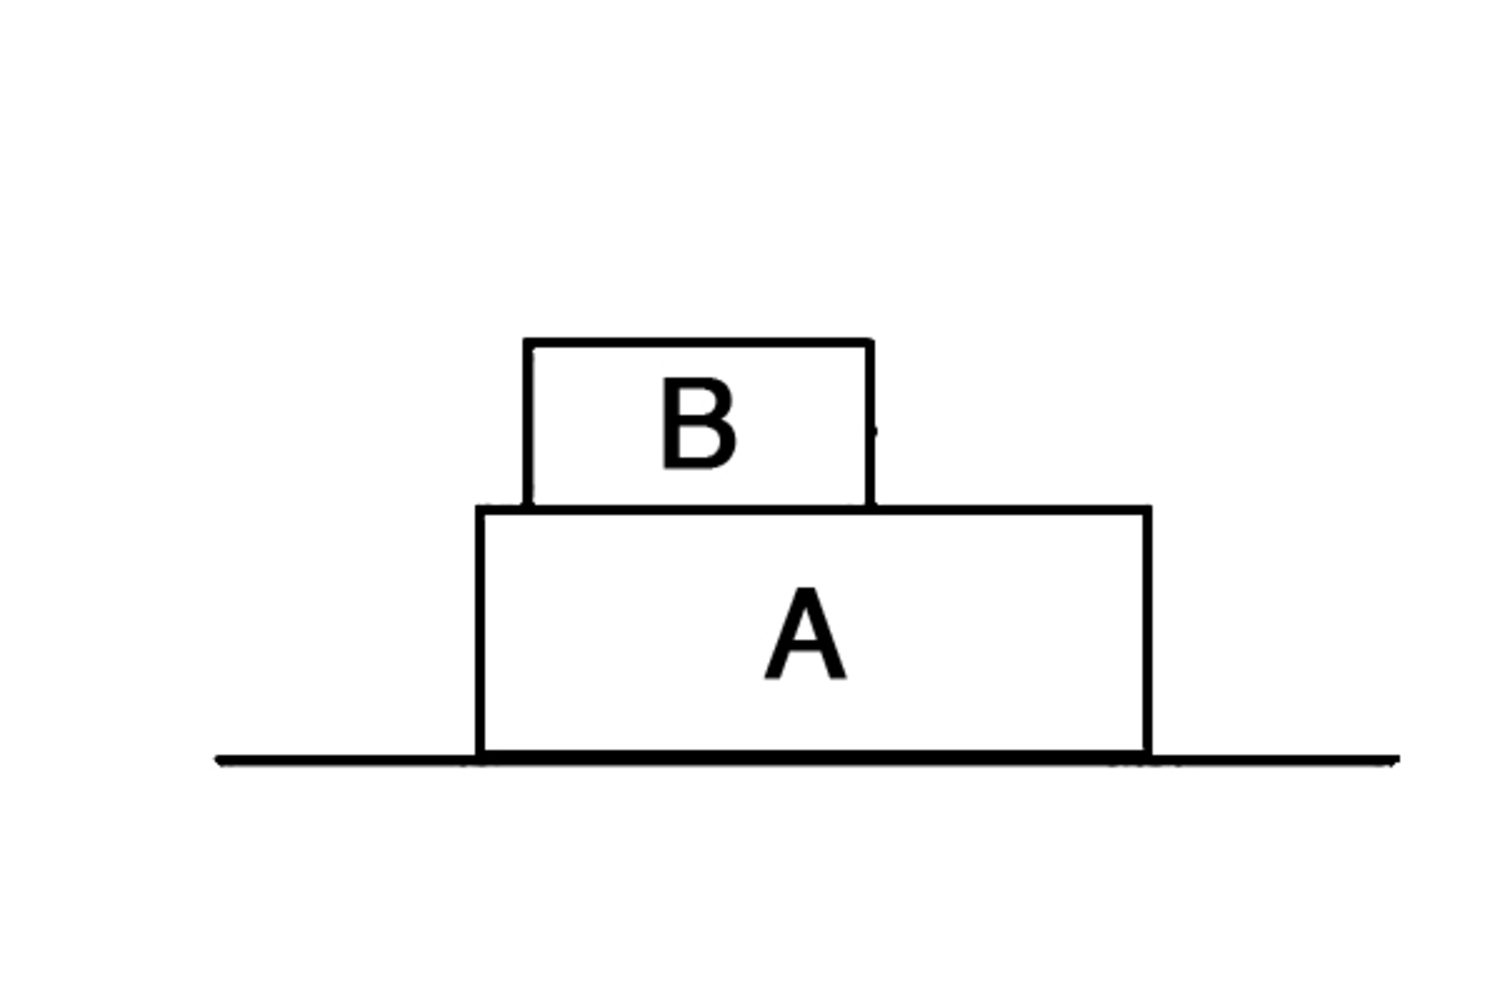
\includegraphics[scale=0.1, clip=true, trim= 20mm 70mm 20mm 110mm]{physics1.jpg}
		\end{figure}
	
		\noindent
		Find \( \displaystyle \frac{m_A}{m_B}  \).
		
		\bigskip
		\noindent
		\textbf{Solution:} \\
		Let $F_{AB}$ be the force exerted by object $A$ to object $B$, and $F_{GA}$ be the force exerted by the plane to object $A$. Thus,
		\begin{equation}
			F_{AB} = m_Bg 	
		\end{equation}
		\begin{equation}
			F_{GA} = \left( m_A + m_B \right) g  = 2F_{AB}	
		\end{equation}
		From (1) and (2), we get
		\[ \left( m_A + m_B \right) g  = 2m_Bg \Rightarrow m_A = m_B \Rightarrow \frac{m_A}{m_B} = \fbox{\textcolor{red}{1}} \]
\end{document}
